\documentclass[
	% -- opções da classe memoir --
	article,			% indica que é um artigo acadêmico
	11pt,				% tamanho da fonte
	oneside,			% para impressão apenas no recto. Oposto a twoside
	a4paper,			% tamanho do papel.
	% -- opções da classe abntex2 --
	%chapter=TITLE,		% títulos de capítulos convertidos em letras maiúsculas
	%section=TITLE,		% títulos de seções convertidos em letras maiúsculas
	%subsection=TITLE,	% títulos de subseções convertidos em letras maiúsculas
	%subsubsection=TITLE % títulos de subsubseções convertidos em letras maiúsculas
	% -- opções do pacote babel --
	english,			% idioma adicional para hifenização
	brazil,				% o último idioma é o principal do documento
	sumario=tradicional
	]{abntex2}


% ---
% PACOTES
% ---

% ---
% Pacotes fundamentais
% ---
\usepackage{lmodern}			% Usa a fonte Latin Modern
\usepackage[T1]{fontenc}		% Selecao de codigos de fonte.
\usepackage[utf8]{inputenc}		% Codificacao do documento (conversão automática dos acentos)
\usepackage{indentfirst}		% Indenta o primeiro parágrafo de cada seção.
\usepackage{nomencl} 			% Lista de simbolos
\usepackage{color}				% Controle das cores
\usepackage{graphicx}			% Inclusão de gráficos
\usepackage{microtype} 			% para melhorias de justificação
% ---
\usepackage{hyperref}
\usepackage{listings}
\usepackage{xcolor}
\usepackage{tcolorbox}
\usepackage{siunitx}
\usepackage{pdfpages}
% ---
% Pacotes adicionais, usados apenas no âmbito do Modelo Canônico do abnteX2
% ---
\usepackage{lipsum}				% para geração de dummy text
% ---

% ---
% Pacotes de citações
% ---
\usepackage[brazilian,hyperpageref]{backref}	 % Paginas com as citações na bibl
\usepackage[alf, abnt-emphasize=bf]{abntex2cite} % Estilo ABNT alfabético% ---

% ---
% Configurações do pacote backref
% Usado sem a opção hyperpageref de backref
\renewcommand{\backrefpagesname}{Citado na(s) página(s):~}
% Texto padrão antes do número das páginas
\renewcommand{\backref}{}
% Define os textos da citação
\renewcommand*{\backrefalt}[4]{
	\ifcase #1 %
		Nenhuma citação no texto.%
	\or
		Citado na página #2.%
	\else
		Citado #1 vezes nas páginas #2.%
	\fi}%
% ---

% --- Informações de dados para CAPA e FOLHA DE ROSTO ---
\titulo{ESTUDO E RESOLUÇÃO DO CICLO DE RANKINE COM MODIFICAÇÕES}
\tituloestrangeiro{}

\autor{
João Alex Arruda da Silva
\\[0.5cm]
Hanna Rodrigues Ferreira}

\local{Brasil}
\data{Fevereiro, 2025}
% ---

% ---
% Configurações de aparência do PDF final

% alterando o aspecto da cor azul
\definecolor{blue}{RGB}{41,5,195}

% informações do PDF
\makeatletter
\hypersetup{
     	%pagebackref=true,
		pdftitle={\@title},
		pdfauthor={\@author},
    	pdfsubject={Modelo de artigo científico com abnTeX2},
	    pdfcreator={LaTeX with abnTeX2},
		pdfkeywords={abnt}{latex}{abntex}{abntex2}{atigo científico},
		colorlinks=true,       		% false: boxed links; true: colored links
    	linkcolor=blue,          	% color of internal links
    	citecolor=blue,        		% color of links to bibliography
    	filecolor=magenta,      		% color of file links
		urlcolor=blue,
		bookmarksdepth=4
}
\makeatother
% ---

% ---
% compila o indice
% ---
\makeindex
% ---

% ---
% Altera as margens padrões
% ---
\setlrmarginsandblock{3cm}{3cm}{*}
\setulmarginsandblock{3cm}{3cm}{*}
\checkandfixthelayout
% ---

% ---
% Espaçamentos entre linhas e parágrafos
% ---

% O tamanho do parágrafo é dado por:
\setlength{\parindent}{1.3cm}

% Controle do espaçamento entre um parágrafo e outro:
\setlength{\parskip}{0.2cm}  % tente também \onelineskip

% Espaçamento simples
\SingleSpacing


% ----
% Início do documento
% ----
\begin{document}

% Seleciona o idioma do documento (conforme pacotes do babel)
%\selectlanguage{english}
\selectlanguage{brazil}

% Retira espaço extra obsoleto entre as frases.
\frenchspacing

% ----------------------------------------------------------
% ELEMENTOS PRÉ-TEXTUAIS
% ----------------------------------------------------------

%---
%
% Se desejar escrever o artigo em duas colunas, descomente a linha abaixo
% e a linha com o texto ``FIM DE ARTIGO EM DUAS COLUNAS''.
% \twocolumn[    		% INICIO DE ARTIGO EM DUAS COLUNAS
%
%---

% página de titulo principal (obrigatório)
\maketitle


% titulo em outro idioma (opcional)



% resumo em português
\begin{resumoumacoluna}
 Conforme a ABNT NBR 6022:2018, o resumo no idioma do documento é elemento obrigatório.
 Constituído de uma sequência de frases concisas e objetivas e não de uma
 simples enumeração de tópicos, não ultrapassando 250 palavras, seguido, logo
 abaixo, das palavras representativas do conteúdo do trabalho, isto é,
 palavras-chave e/ou descritores, conforme a NBR 6028. (\ldots) As
 palavras-chave devem figurar logo abaixo do resumo, antecedidas da expressão
 Palavras-chave:, separadas entre si por ponto e finalizadas também por ponto.

 \vspace{\onelineskip}

 \noindent
 \textbf{Palavras-chave}: latex. abntex. editoração de texto.
\end{resumoumacoluna}

% ----------------------------------------------------------
% ELEMENTOS TEXTUAIS
% ----------------------------------------------------------
\textual

% ----------------------------------------------------------
% Introdução
% ----------------------------------------------------------
\section{Introdução}

Segundo \cite{moran-2018}, o ciclo de Rankine é a estrutura fundamental das usinas termelétricas que operam com vapor. Este é um dos principais ciclos termodinâmicos utilizados na engenharia mecânica para conversão de calor em trabalho, sendo a base para o funcionamento de usinas termoelétricas e outras instalações de geração de energia. Esse ciclo opera com um fluido de trabalho, geralmente água, que passa por processos de aquecimento, expansão, resfriamento e compressão.

Para melhorar a eficiência do Ciclo de Rankine, diversas modificações são adotadas, como o superaquecimento, o reaquecimento e o uso de ciclos supercríticos. Essas modificações têm o objetivo de aumentar a eficiência térmica e reduzir perdas energéticas, tornando as plantas de geração mais sustentáveis e econômicas.

Este trabalho pretende analisar detalhadamente o ciclo de Rankine e suas variações, visando aprofundar o conhecimento sobre sistemas térmicos voltados à produção de energia. Para isso, será realizada uma revisão teórica robusta dos princípios termodinâmicos envolvidos, seguida da aplicação desses conceitos em um estudo de caso prático, que abordará técnicas como reaquecimento, expansão em dois estágios e regeneração térmica.

\section{Revisão bibliográfica}

\subsection{Definição do ciclo de Rankine}

O Ciclo de Rankine é um ciclo termodinâmico idealizado que descreve o funcionamento de uma usina termelétrica convencional. Esse ciclo é composto por quatro processos termodinâmicos: compressão, aquecimento, expansão e resfriamento. A Figura \ref{fig:esquema-simplificado-ciclo-rankine} ilustra o diagrama de um ciclo de Rankine básico.

\begin{figure}[h]
	\centering
	\caption{Esquema simplificado e o diagrama T-S do ciclo Rankine}
	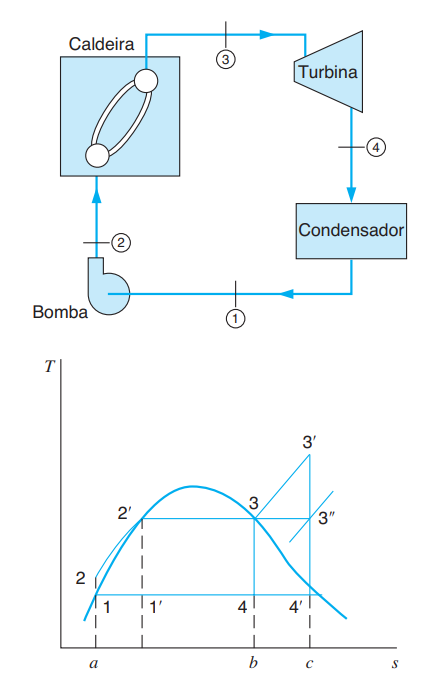
\includegraphics[width=0.7\textwidth]{./images/Esquema simplificado e o diagrama T-S do ciclo Rankine.png}
	\label{fig:esquema-simplificado-ciclo-rankine}
	\fonte{Adaptado de \cite{borgnakke-2020}}
\end{figure}

O fluido de trabalho fica sujeito à seguinte sequência de processos reversíveis internamente: \cite{borgnakke-2020}

\begin{itemize}
	\item \textbf{Processo 1-2}: Processo de bombeamento adiabático reversível na bomba.
	\item \textbf{Processo 2-3}: Transferência de calor a pressão constante na caldeira.
	\item \textbf{Processo 3-4}: Expansão adiabática reversível na turbina (ou em outra máquina motora, tal como a máquina a vapor).
	\item \textbf{Processo 4-1}: Transferência de calor a pressão constante no condensador.
\end{itemize}

Ao desconsiderar as variações de energia cinética e potencial, as trocas de calor e o trabalho líquido do sistema podem ser visualizados como áreas específicas no diagrama temperatura-entropia (T-s). O calor absorvido pelo fluido de trabalho corresponde à área delimitada pelos pontos a-2-2'-3-b-a, enquanto o calor rejeitado pelo fluido é representado pela área a-1-4-b-a. Aplicando a primeira lei da termodinâmica, conclui-se que o trabalho líquido é equivalente à diferença entre essas duas áreas, ou seja, corresponde à região 1-2-2'-3-4-1 no diagrama \cite{borgnakke-2020}.

Na análise do ciclo Rankine, é útil considerar que o rendimento depende da temperatura média na qual o calor é fornecido e da temperatura média na qual o calor é rejeitado. Qualquer variação que aumente a temperatura média na qual o calor é fornecido, ou que diminua a temperatura média na qual o calor é rejeitado, aumentará o rendimento do ciclo Rankine.

\subsection{Componentes Básicos}

Independentemente de um modelo detalhado ou simplificado de usina a vapor baseada no ciclo Rankine, os fundamentos termodinâmicos (conservação de massa/energia, segunda lei e dados termodinâmicos) aplicam-se tanto aos componentes individuais (turbinas, bombas, trocadores de calor) quanto ao ciclo global.

Focando no subsistema mostrado na Figura \ref{fig:planta-exemplo}, modelam-se os quatro componentes principais: turbina, condensador, bomba e caldeira, com água como fluido de trabalho. Usinas a combustíveis fósseis são analisadas como referência, mas os princípios valem para outros tipos.

\begin{figure}[h]
	\centering
	\caption{Planta de potência a vapor acionada por combustível fóssil}
	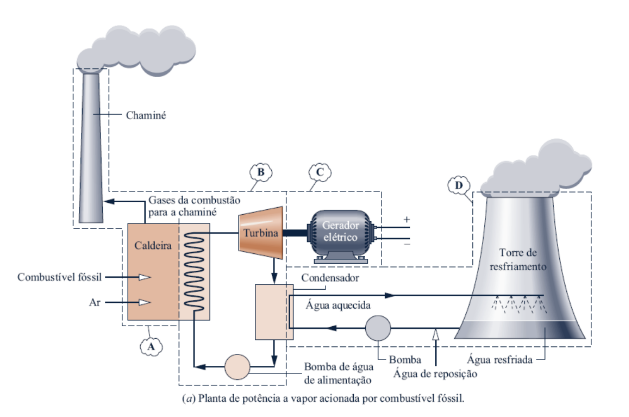
\includegraphics[width=1.0\textwidth]{./images/planta-exemplo.png}
	\label{fig:planta-exemplo}
	\fonte{\
	cite{moran-2018}}
\end{figure}

No diagrama da Fig. 2, trabalho e calor são positivos conforme as setas, para simplificar a análise usamos algumas hipóteses frequentes, conforme descrito abaixo:
\begin{itemize}
	\item R. P. em todos os componentes.
	\item Energia potencial e cinética desprezível.
    \item Perdas de pressão na caldeira e no condensador desprezíveis.
    \item Bombas e turbinas são consideradas isentrópicas.
\end{itemize}

Será mostrado a seguir a modelagem do ciclo para cada componente do ciclo Rankine, conforme é exibido por \citeonline{moran-2018}

\subsubsection{Turbina}

A turbina é o componente que converte a energia térmica do vapor em trabalho mecânico. O vapor entra na turbina com uma pressão e temperatura elevadas e sai com pressão e temperatura menores. O trabalho líquido da turbina é a diferença entre o trabalho de entrada e saída, conforme a equação \ref{eq:trabalho-turbina}.

\begin{equation}
	\dot{W}_{\text{turbina}} = \dot{m}(h_1 - h_2)
	\label{eq:trabalho-turbina}
\end{equation}

\subsubsection{Condensador}

O condensador é o componente que converte o vapor em água líquida, rejeitando calor para o ambiente. O calor rejeitado pelo condensador é a diferença entre o calor de entrada e saída, conforme a equação \ref{eq:calor-condensador}.

\begin{equation}
	\dot{Q}_{\text{condensador}} = \dot{m}(h_2 - h_3)
	\label{eq:calor-condensador}
\end{equation}

\subsubsection{Bomba}

A bomba é o componente que comprime a água líquida, aumentando sua pressão. O trabalho líquido da bomba é a diferença entre o trabalho de entrada e saída, conforme a equação \ref{eq:trabalho-bomba}.

\begin{equation}
	\dot{W}_{\text{bomba}} = \dot{m}(h_4 - h_3)
	\label{eq:trabalho-bomba}
\end{equation}

\subsubsection{Caldeira}

A caldeira é o componente que converte a água líquida em vapor, absorvendo calor do ambiente. O calor absorvido pela caldeira é a diferença entre o calor de entrada e saída, conforme a equação \ref{eq:calor-caldeira}.

\begin{equation}
	\dot{Q}_{\text{caldeira}} = \dot{m}(h_1 - h_2)
	\label{eq:calor-caldeira}
\end{equation}

\subsection{Parâmetros de Desempenho}

A eficiência térmica do ciclo Rankine é dada pela razão entre o trabalho líquido produzido e o calor fornecido na caldeira, conforme a equação \ref{eq:eficiencia-termica}.

\begin{equation}
	\eta = \frac{\dot{W}_{\text{turbina}}}{\dot{Q}_{\text{caldeira}}}
	\label{eq:eficiencia-termica}
\end{equation}

% ---
% Finaliza a parte no bookmark do PDF, para que se inicie o bookmark na raiz
% ---
\bookmarksetup{startatroot}%
% ---

% ---
% Conclusão
% ---
\section{Considerações finais}

% ----------------------------------------------------------
% ELEMENTOS PÓS-TEXTUAIS
% ----------------------------------------------------------
\postextual

% ----------------------------------------------------------
% Referências bibliográficas
% ----------------------------------------------------------
\bibliography{references}


\end{document}
